\chapter{Materiais e Métodos}
\label{chap:mat}
A metodologia de execução e gerenciamento aplicada no projeto ELIR é baseada na metodologia empregada na área de robótica do SENAI CIMATEC. O projeto foi dividido em três fases principais para facilitar a organização e gerenciamento das atividades. O diagrama com as fases do projeto está mostrado na Figura \ref{Fig:flux_proj}.

\begin{figure}[h]
	\centering
	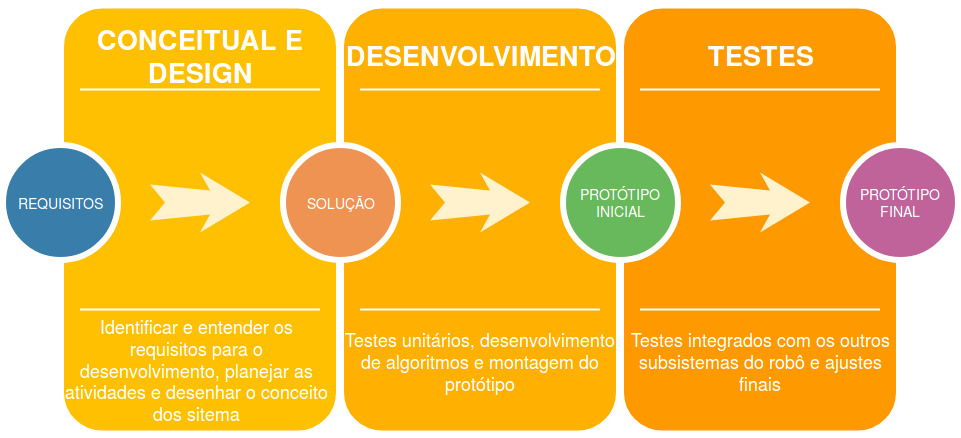
\includegraphics[width=16cm]{Figures/diagrama_proj.jpg}
	\caption{Fluxograma do Projeto}
	\label{Fig:flux_proj}
\end{figure}

% sugiro diminuir as letras do título de cada fase na figura, a palavra SOLUÇÃO não está adequada, conforme já havia falado pra ti

\section{Conceitual e Design}

A fase de Conceitual e Design é marcada por uma série de reuniões de alinhamento com o orientador do projeto e cliente, a fim de definir os requisitos técnicos do projeto, os materiais a serem utilizados, as funcionalidades do sistema, a arquitetura geral da Percepção e a arquitetura de software empregada. Esta é a etapa de criação do conceito tecnológico além de organização e planejamento das atividades. 
%precisa explicar o que é esta fase e não descrevê-la

\subsection{Requisitos técnicos}

%o trabalho agora é um TCC e não um relatório, na metodologia vc deve descrevê-la
Os requisitos técnicos do projeto foram definidos nas primeiras reuniões com o orientador do projeto. Estes requisitos foram elaborados com base nos requisitos do cliente e estão mostrados abaixo:


\begin{itemize}
	\item{\textbf{Inspeção de Temperatura dos cabos, estrutura e obstáculos}}: Devem ser disponibilizadas as informações de medição de temperatura dos cabos, estrutura da linha e de seus obstáculos. Esses dados devem ser obtidos através da câmera térmica para inspeção
	\item{\textbf{Georreferenciamento dos eventos}}: Todos os eventos de detecção de pontos quentes, sobretemperatura e sobrecorrente devem ser sinalizados em um \textit{logfile} informando a data, horário e coordenadas geográficas obtidos pelo GPS.
	\item{\textbf{Disponibilizar os videos dos eventos}}: A inspeção realizada pela câmera térmica deve ser disponibilizada em tempo real na interface gráfica do robô.
	\item{\textbf{Identificação de posicionamento da garra no cabo}}: A fim de garantir a confiabilidade da operação, deve ser realizado uma verificação do alinhamento das garras no cabo da linha de alta tensão.
	\item{\textbf{Inspeção da linha de servidão}}: Devem ser disponibilizadas informações de objetos até sete metros abaixo do robô
	\item \textbf{Monitorar temperatura do protótipo}: A temperatura da parte interna do protótipo deve ser monitorada para garantir a segurança dos equipamentos eletrônicos presentes.
\end{itemize}

\subsection{Lista de materiais}
% precisa explicar a metodologia este assunto é do desenvolvimento
No sistema de Percepção os sensores atuam como os sentidos do robô, recebendo dados externos e informando a unidade central de processamento os seus significados. Quanto maior o número de grandezas físicas analisadas, mais complexo o sistema de Percepção e maior a sua capacidade de compreensão. 

Os sensores que compõem o sistema de Percepção do robô ELIR foram escolhidos com base nas necessidades de cada funcionalidade do sistema e disponibilidade do componente na própria instituição. A lista de componentes utilizada está mostrada na Figura \ref{fig:list_mat}. Os preços mostrados não refletem o custo do projeto uma vez que os materiais utilizados são pertencentes ao SENAI CIMATEC. Os valores mostrados são preços médios do produto encontrados na página dos fornecedores. 

\begin{figure}[h]
	\centering
	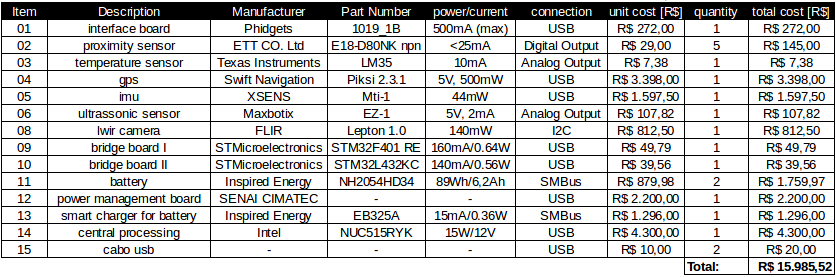
\includegraphics[width=16cm]{Figures/lista_materiais.png}
	\caption{Lista de materiais utilizados no sistema de Percepção do robô ELIR}
	\label{fig:list_mat}
\end{figure}

\subsubsection{Descrição dos componentes}

A Phidgets é uma placa de interface que concentra os dados provenientes de suas portas digitais, analógicas e USBs em uma única porta USB. Ela atua como um hub concentrando todas as informações em um único local . No ELIR a placa é utilizada para concentrar as informações do sonar, sensores de proximidade,  baterias, GPS e IMU em uma única porta USB a ser conectada na unidade central de processamento. A sua utilização é importante por conta da limitação de portas USBs na unidade de processamento central.

As placas Nucleo STM32F401RE  e   Nucleo STM32L432 são placas de desenvolvimento para aplicações utilizando o microprocessador ARM. No ELIR a placa Nucleo STM32F401RE é utilizada para converter os dados provenientes da câmera térmica em protocolo SPI para o protocolo USB. A familia  F4 foi utilizada pois pode atingir clocks de 20GHz, é necessario um microprocessador que consiga atingir esta faixa de clock para ter sincronia com o módulo da câmera. A placa possui um canal de comunicação exclusivo com a unidade central de processamento. 

Já a placa  Nucleo STM32L432 é utilizada para conversão das informações provenientes das baterias em protocolo SMBus para o protocole USB. Esta placa é conectada a uma porta USB da Phidgets. Para a execução desta atividade não é necessário um microprocessador de alto desempenho e por isso a família L4 foi escolhida por ter  baixo consumo de energia.

O sensor E18D80-NK é um sensor de proximidade infravermelho, ele é utilizado no ELIR para identificar se as garras do robô estão apoiadas na linha de transmissão. A saída do sensor é digital e o estado do pino  de dados indica a presença ou ausência de um objeto. Foi realizada uma pesquisa dos sensores de proximidade no mercado e este sensor foi escolhido por ser de baixo custo, compacto e pode ser utilizado em superfícies metálicas. 

O sensor EZ1 da MaxBotix é um sonar. Ele é utilizado no projeto para monitorar objetos dentro da faixa de servidão. Foi utilizado o EZ1 por ele cumprir com os requisitos do cliente do alcance da área de servidão.

O sensor de temperatura LM35 é utilizado no projeto para medição da temperatura na estrutura interna do robô. Ele foi escolhido por ter reposta linear e ser de baixo custo.

O GPS SwiftNav Piksi é utilizado no projeto para obter informações de latitude e longitude quando detectado alguma anormalidade. Enquanto a IMU Xsens Mti-1 é utilizada no projeto para obter informaçoes dos ângulos de orientação do robô. Estes módulo são superdimensionado para a aplicação inicial do projeto, ainda assim os mesmos foram utilizados por terem disponibilidade na instituição e possuirem drivers para o ambiente ROS disponibilizados pelo fabricante.

As bateriais NH2054 da Inspired Energy são células de 14V para alimentação do sistema de Percepção. Elas são baterias inteligente que fornecem informações de temperatura, tensão, corrente e capacidade das células. Foram escolhidas pela quantidade de informações que podem fornecer.

A Power Management Board é uma placa de gerenciamento de energia do sistema robótico, ela distribui a tensão proveniente das baterias para todos os sensores. 

A intel NUC 515RYK é a unidade de processamento central do sistema de Percepção, ela recebe as informações de todos os sensores dos sitema de Percepção e os interpreta. 



\subsection{Funcionalidades do Sistema}


As funcionalidades de um robô descrevem os subsistemas e a lógica de operação dos mesmos. No ELIR, o sistema de Percepção possui três funcionalidades principais: Aquisição, Localização e Detecção. A descrição de cada funcionalidade e seu diagrama de funcionamento estão mostrados nos subtópicos a seguir. 

\subsubsection{Aquisição}
\label{ssec:func1}

O processo de aquisição de dados envolve a comunicação dos sensores com seus respectivos drivers no ambiente ROS e a disponibilização dos dados para as outras funcionalidades do sistema.

Os sensores analógicos e digitais terão seus dados tratados pelo driver da interface Phidgets no ambiente ROS. Para os dispositivos relacionados a localização como o GPS e a IMU, serão utilizado drivers já disponibilizados pelos fabricantes.

No caso dos componentes que trabalham com os protocolos de comunicação SPI ou I2C, como é o caso da câmera térmica e da \textit{Smart Charger}, serão utilizadas duas interfaces baseadas em ARM com um \textit{firmware} embarcado para a conversão dos dados para o protocolo UART.

A interface microprocessada utilizada para obter dados da câmera térmica possui uma porta USB dedicada na unidade de processamento Intel NUC. Já a outra interface microprocessada para a \textit{Smart Charger} será conectada a uma porta USB da Phidgets.

No ambiente ROS do projeto há um \textit{package} exclusivo para receber os dados convertidos da câmera térmica, um \textit{package} para receber dados de todos os sensores conectados a Phidgets, um \textit{package} para recebimento de dados da \textit{Smart Charger} e por último um \textit{package} exclusivo para interface gráfica. 
Pode-se observar o fluxograma da aquisição na Figura %\ref{FuncAquisition}

\begin{figure}[!ht]
	\centering
	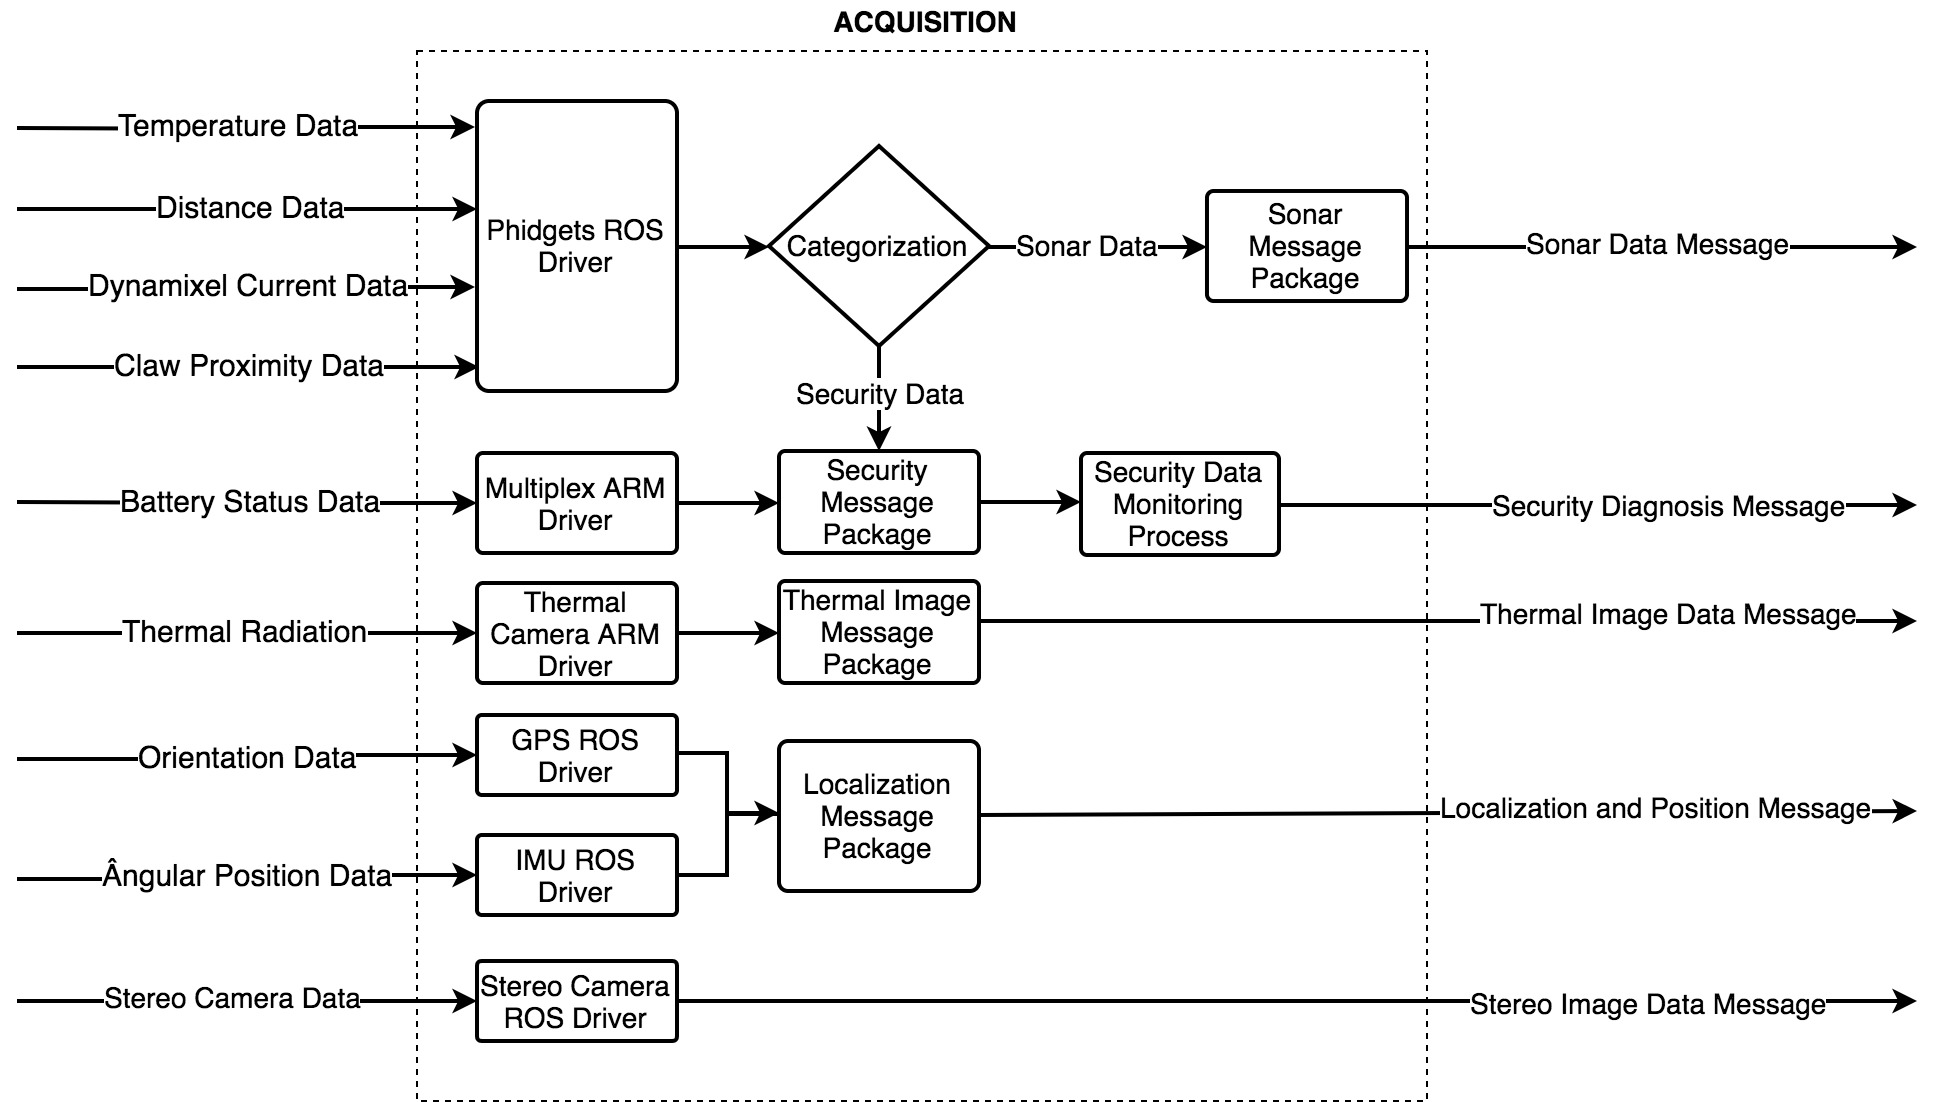
\includegraphics[height=7cm, width=14cm]{Figures/Fluxograma_Aquisition.jpg}
	\caption{Fluxograma da Funcionalidade Aquisição} \label{FuncAquisition}
\end{figure}

Para correta execução desta funcionalidade é necessário o funcionamento dos sensores segundo o nível de prioridade dos mesmos. Logo, um estudo de casos de falhas para cada sensor foi realizado, no qual foi definido um nível de criticidade de acordo com o impacto de sua função no sistema como um todo. Foram elaborados três níveis de criticidade:
\begin{itemize}
	\item Level 1 - Sensores com impacto crítico na operação. Em casos de falha, a inspeção não poderá ser realizada.
	\item Level 2 - Sensores com impacto médio na operação. Em caso de falha, a inspeção poderá ser realizada de forma parcial.
	\item Level 3 - Sensores com impacto leve na operação. Em caso de falha, não haverá dados de monitoramento da situação de temperatura e consuno energético do robô, porém a inspeção poderá continuar normalmente.
\end{itemize}

Na figura abaixo, pode-se observar os sensores e suas categorias.

\begin{figure}[!ht]
	\centering
	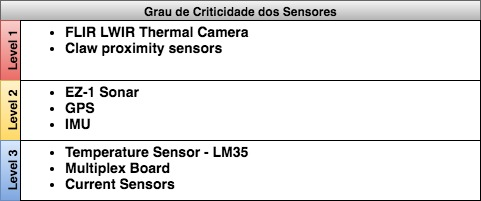
\includegraphics[height=7cm, width=14cm]{Figures/criticidade.jpg}
	\caption{Nível de criticidade dos sensores} \label{FuncAquisition}
\end{figure}

\subsubsection{Objetivo}
Realizar a comunicação e a aquisição dos dados provenientes da câmera térmica, sensores de proximidade, sonar, GPS, IMU, sensor de temperatura, \textit{Smart Charger} e sensores de corrente.

\subsubsection{Dependências}
Esta funcionalidade não depende de nenhum outro processo.

\subsubsection{Premissas}
\begin{itemize}
	\item A interface microcontrolada Nucleo STM32F401RE deve estar com firmware embarcado para conversão de dados SPI para UART.
	\item A câmera térmica deverá estar conectada à interface Nucleo STM32F401RE
	\item A câmera stereo deve está conectada à NUC através da porta USB
	\item O sensores de temperatura, corrente e sonar devem estar conectados as entradas analógicas da interface Phidgets
	\item Os sensores de proximidade devem está conectados as entradas digitais da placa de interface Phidgets
	\item O GPS e a IMU devem estar conectados a portas USB da Phidgets
	\item As placas de interface devem estar energizadas.
\end{itemize}

\subsubsection{Saídas}

Esta funcionalidade possui quatro saídas:

\begin{itemize}
	\item \textit{Sonar Data Message}: Mensagem de saída exclusiva para os dados do sonar EZ-1.
	\item \textit{Secutiry Diagnose Message}: Mensagem contendo todos os dados relacionados à segurança e integridade do robô.
	\item \textit{Thermal Image Data Message}: Mensagem exclusiva para os dados da câmera térmica.
	\item \textit{Localization and Position Message}: Mensagem contendo os dados relacionados á localização e posicionamento angular do robô.
\end{itemize}

\subsubsection{Localização}
\label{ssec:func2}

O sistema de localização envolve o monitoramento da posição latitudinal e longitudinal do robô, assim como a posição angular através do GPS e da IMU respectivamente.

A localização é um package que ao receber uma requisição de informação, coleta os dados de posicionamento e orientação do robô provenientes do sistema de Aquisição e encaminha para o sistema que requisitou.

O fluxograma deste funcionalidade pode ser visto na Figura \ref{fluxlocal}

\begin{figure}[h!]
	\centering
	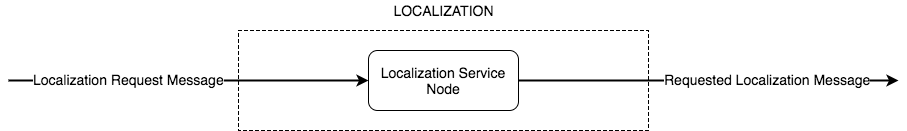
\includegraphics[width=16cm]{Fluxograma_Localization.png}
	\caption{Fluxograma da Funcionalidade Localização} \label{fluxlocal}
\end{figure}


\subsubsection{Objetivo}
O objetivo desta funcionalidade é disponibilizar os dados de Localização do robô no ambiente ROS para a funcionalidade de Detecção.

\subsubsection{Dependências}
O sistema de localização depende dos dados de posicionamento e orientação disponibilizados pelo sistema de Aquisição.

\subsubsection{Premissas}
\begin{itemize}
	\item O sistema de Aquisição deve está funcionando corretamente até o Nível 2 de criticidade dos sensores.
	\item GPS e IMU estão posicionados em uma estrutura rígida e com o menor vibração possível.
\end{itemize}

\subsubsection{Saídas}

\begin{itemize}
	\item \textit{Requested Localization Message}: Mensagem que informa os dados de localização para o sistema que os requisitou.
\end{itemize}

\subsubsection{Detecção}
\label{ssec:func3}

A detecção é a funcionalidade responsável por identificar a presença de pontos quentes na linha de transmissão bem como de objetos na faixa de servidão. Ao identificar um destes elementos, o sistema solicita da funcionalidade de Localização os dados posicionamento e orientação do robô e envia uma mensagem de alerta.

A mensagem de detecção de um ponto quente informa a localização do robô e a localização do objeto no frame de imagem. Por isso recebe a mensagem de detecção de obstáculos. 

A mensagem de detecção de objetos na faixa de servidão informa a distância da cota da linha até o objeto e a localização do mesmo. 

\subsubsection{Objetivo}

O objetivo desta funcionalidade é coletar as informações provenientes da câmera infravermelha e do sonar, como presença de pontos quentes e objetos presentes na área de servidão. 

\subsubsection{Dependências}
O sistema de detecção depende dos dados do sonar e dos \textit{frames} da câmera térmica disponibilizados pelo sistema de Aquisição. Além disto, depende do sistema de Localização para adquirir informações de posicionamento e orientação do robô.

\subsubsection{Premissas}
\begin{itemize}
	\item O sistema de Aquisição deve está funcionando corretamente até o Nível 2 de criticidade dos sensores.
	\item GPS e IMU estão posicionados em uma estrutura rígida e com o menor vibração possível.
	\item A câmera térmica deve estar calibrada e posicionada com ângulo de visão para as linhas de transmissão e seus obstáculos
	\item O sonar deve estar posicionado de forma a monitorar objetos abaixo da linha de transmissão.            
\end{itemize}

\begin{figure}[!ht]
	\centering
	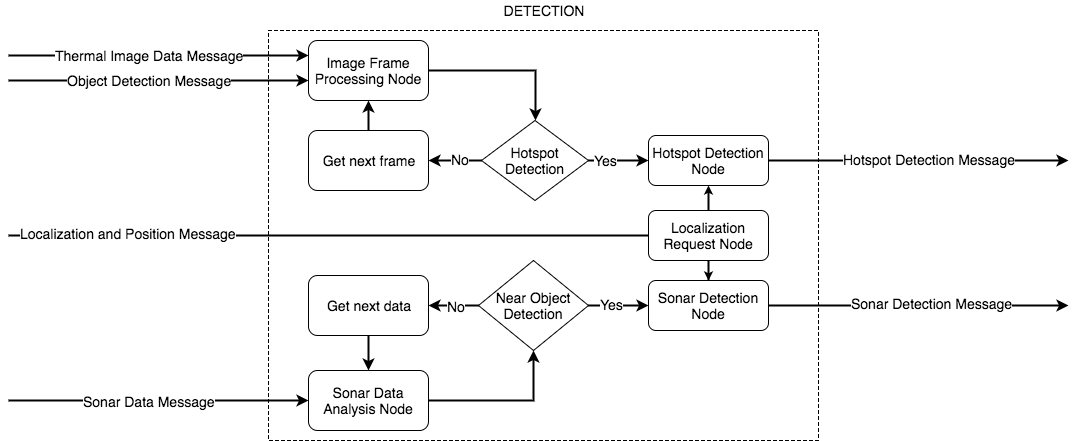
\includegraphics[width=16cm]{Fluxograma_Detection.png}
	\caption{Fluxograma da Funcionalidade Detecção} \label{FuncDetec}
\end{figure}

\subsubsection{Saídas}

\begin{itemize}
	\item \textit{Hotspot Detection Message}: Mensagem que informa a detecção de um ponto quente e informa a sua localização na imagem e localização do robô na linha.
	\item \textit{Sonar Detection Message}: Mensagem que informa a detecção de objetos na faixa de servidão e sua localização na linha.
	%\item Localization Request Message: Mensagem de requisição dos dados posicionamento e orientação do robô para o sistema de Localização
\end{itemize}
	
	\section{Desenvolvimento}
	Na fase de Desenvolvimento são realizados os testes unitários dos sensores do sistema de Percepção, a implementação de protocolos de comunicação, integração dos sensores no framework de robótica ROS e desenvolvimento da interface gráfica. O resultado principal desta fase é a conexão dos sensores em rede no framework de robótica e a interface gráfica exibindo em tempo real as informações mais relevantes do sistema de Percepção.
	%tem que explicar o que esta fase
	
	\subsection{Testes Unitários}
	
	\begin{itemize}
		\item Câmera Térmica
		
		A câmera térmica Lepton, do fabricante FLIR, se comunica por VOSPI. Logo, foi necessário utilizar um driver para converter os dados da câmera e disponibiliza-los para a USB. Uma placa de desenvolvimento Nucleo STM32F401RE com o driver disponibilizado por \citeonline{groupgets} foi utilizada para essa situação.
		
		\begin{figure}[!ht]
			\centering
			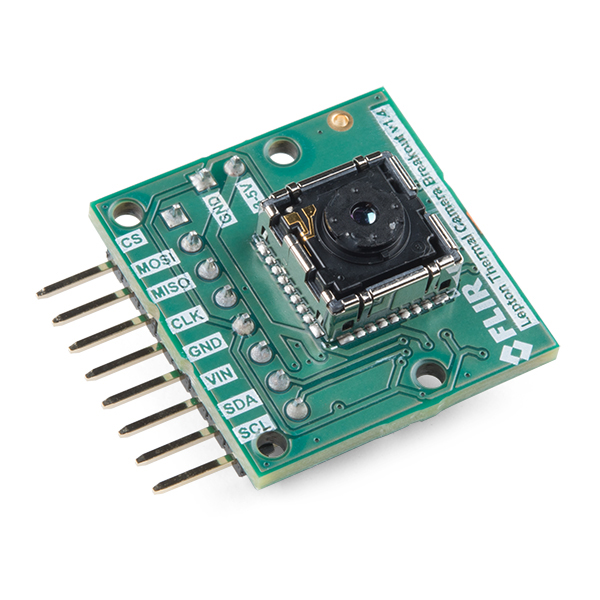
\includegraphics[width=6cm]{Figures/lepton_flir.jpg}
			\caption{Lepton LWIR}
			\label{fig:lepton}
		\end{figure}
		
		O driver coleta os frames e verifica se o mesmo foi adquirido corretamente, após isso, envia para a USB seguindo o seguinte padrão de mensagem:
		
		\begin{figure}[!ht]
			\centering
			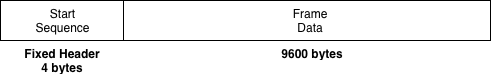
\includegraphics[width=14cm]{Figures/frame_msg.png}
			\caption{Mensagem do frame da câmera}
			\label{fig:framemsg}
		\end{figure}
		
		No início de cada mensagem, há uma sequência de quatro \textit{bytes} para confirmar a transferência dos dados. Após a confirmação por um \textit{script} em python, inicia-se o processo de aquisição do \textit{frame}. Cada \textit{frame} é composto por 4800 \textit{pixeis}, sendo 80 na horizontal e 60 na vertical. Além disso, cada \textit{pixel} possui 2 \textit{bytes} de profundidade de cor, correspondendo a 9600 \textit{bytes} de informação para cada \textit{frame}. Na Figura \ref{fig:frame_esque}, pode-se observar uma representação do \textit{frame} da câmera.
		
		%\pagebreak
		
		\begin{figure}[!ht]
			\centering
			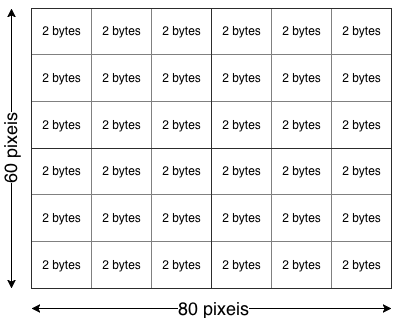
\includegraphics[width=10cm]{Figures/frame_esque.png}
			\caption{Esquemático do \textit{Frame} da Câmera Térmica}
			\label{fig:frame_esque}
		\end{figure}
		
		No \textit{script} de aquisição de \textit{frames}, cada \textit{pixel}, foi convertido para uma escala de cinza de 8-bits (1 \textit{byte}). Conversão necessária para trabalhar com a biblioteca de processamento de imagens OpenCV.
		
		Após isso a imagem foi reconstruída para verificar a integridade dos \textit{frames}.
		
		\item Sonar EZ-1
		
		O sonar EZ-1 da MaxBotix possui saída analógica referente a distância medida. Para testa-lo, foi utilizada uma das entradas analógicas da Phidgets.
		
		\pagebreak
		
		\begin{figure}[!ht]
			\centering
			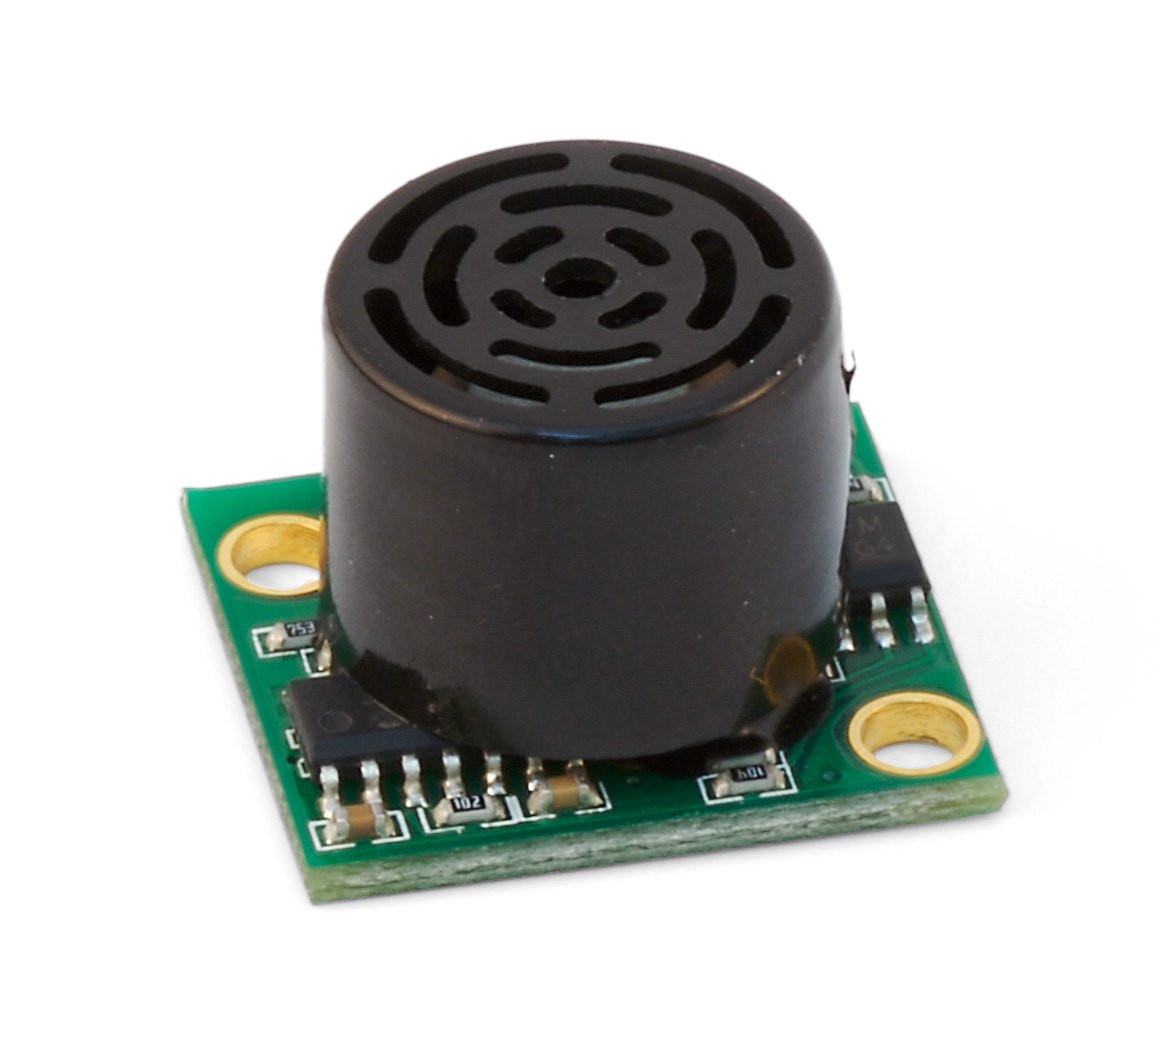
\includegraphics[width=8cm]{Figures/ez1.jpg}
			\caption{Sonar EZ-1}
			\label{fig:ez1}
		\end{figure}
		
		A comunicação da Phidgets com com a NUC é feita via USB, contudo, é necessário a instalação dos drivers obrigatórios da placa no linux. Além disso, é necessário a instalação do módulo python respectivo da placa, dessa forma, permitindo a utilização de classes e métodos para controle da comunicação com os sensores.
		
		Com os respectivos drivers e módulos da phidgets instalados no computador, foi necessário apenas conectar os terminais alimentação e saída analógica do sensor nos conectores correspondentes da Phidgets e executar um \textit{script} de leitura da tensão nas entradas analógicas fornecido pela própria fabricante. 
		
		Ao executar o código, recebe-se, no intervalo de dez segundos, todas as leituras de tensão efetuadas no sensor. Notamos que ao afastar o obstáculo do sonar o valor de tensão aumentava e quando aproximavamos o obstáculo o valor de tensão diminuía. Após feita a conversão de tensão para unidades métricas através das informações disponibilizadas no \textit{datasheet}, foi possível validar o sensor.
		
		\item Sensor de Proximidade
		
		O sensor de proximidade E18-D80NK funciona de maneira bastante simples. O módulo possui um emissor e um receptor de feixes infra-vermelhos, o qual identifica se há ou não um objeto próximo devido a reflexão, liberando assim, um sinal de nível alto caso positivo e nível baixo caso negativo.
		
		\begin{figure}[!ht]
			\centering
			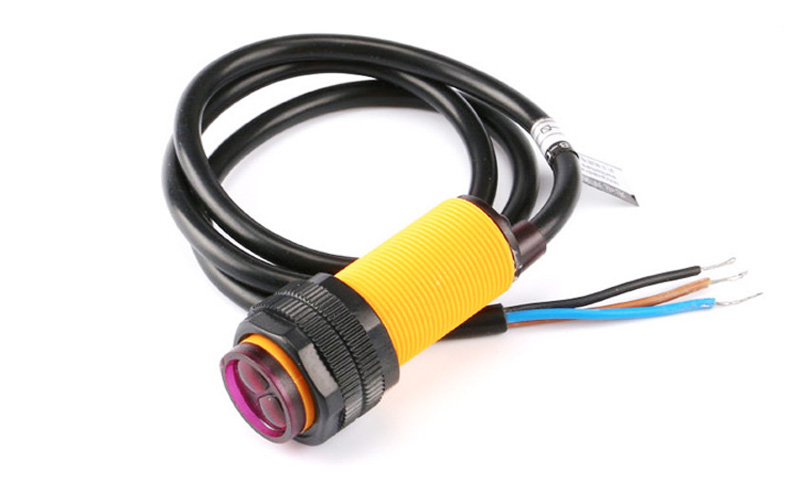
\includegraphics[width=8cm]{Figures/proximity_sensor.jpg}
			\caption{Sensor de proximidade E18-D80NK}
			\label{fig:E18-D80NK}
		\end{figure}
		
		Por questão de sinalização, o fabricante adicionou um LED, que ao identificar algum objeto próximo, acende-se. Com isso, logo após alimentar o sensor já era possível ver o seu funcionamento. Entretanto, ainda era necessário verificar se a saída digital referente a detecção estava em devido funcionamento.
		
		Para isso, foi utilizada a placa de interfaceamento Phidgets assim como no tópico anterior. O que diferiu nesse teste para o anterior é que o sensor foi acoplado em uma entrada digital, em vez de uma analógica, assim como o \textit{script} executado foi para comunicação com as entradas digitais. O código, também disponibilizado pela fabricante, notifica a mudança de estado da saída dos sensor, dessa maneira podendo ser validada.
		
		\item \textit{Smart Charger}
		
		A placa de gerenciamento e carregamento das baterias DS325A, da empresa Inspired Energy, funciona a partir do protocolo de comunicação SMBus. Informações das baterias como temperatura, corrente, carga, entre outras podem ser solicitadas através do seguinte protocolo de leitura.
		
		\begin{figure}[!ht]
			\centering
			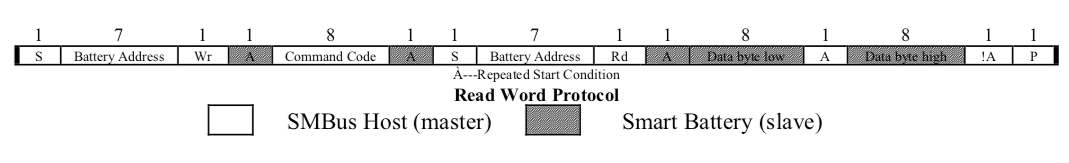
\includegraphics[width=16cm]{Figures/batt_protocol.png}
			\caption{Protocolo de comunicação do \textit{Smart Charger} e das baterias}
			\label{fig:batt_protocol}
		\end{figure}   
		
		No qual é necessário enviar primeiro o endereço de 7 bits da bateria de interesse, seguido do comando referente a que informação está se requisitando. Após isso, inicia-se o processo de leitura das informações da bateria.
		
		O driver de comunicação foi desenvolvido em uma placa de desenvolvimento Nucleo STM3L432KC para disponibiliza-los na USB do computador. Além disso, um \textit{script} em python foi escrito para requisitar essas informações do microcontrolador.
		
		Os dados foram convertidos para suas respectivas grandezas, dessa maneira, foi possível validar as informações obtidas.
		
		\item Sensor de Temperatura
		
		O sensor de temperatura LM35 possui uma saída analógica e com comportamento linear entre a tensão de saída e a temperatura medida.
		
		\begin{figure}[!ht]
			\centering
			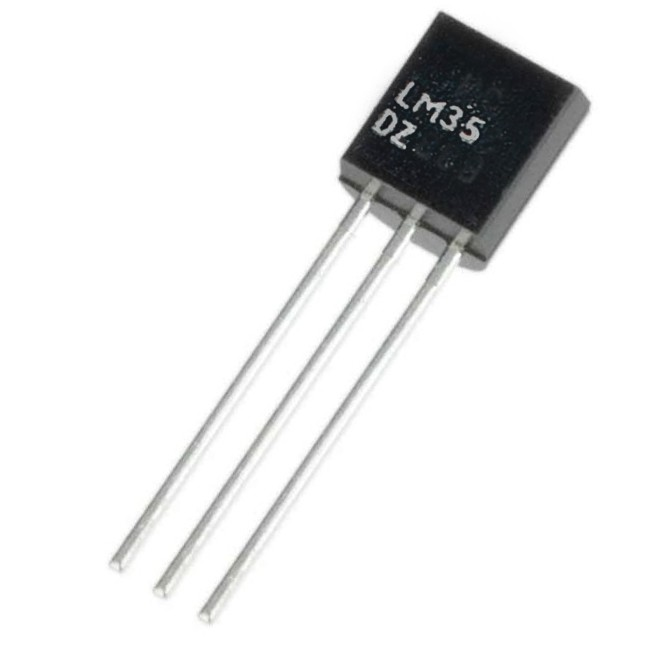
\includegraphics[width=6cm]{Figures/lm35.jpg}
			\caption{Sensor de Temperatura LM35}
			\label{fig:LM35}
		\end{figure}
		
		O componente foi testado em uma das entradas analógicas da Phidgets, e utilizando o mesmo algoritmo de leitura de tensão já mencionado para realizar a obtenção de dados. Para verificar a resposta do sensor, foi medido o valor de tensão de saída para uma sala com ar-condicionado e para um ambiente externo com auxílio de um termômetro de referência.
		
		Os valores de tensão foram convertidos para graus Celsius, através da correlação disponível no \textit{datasheet}, validando assim o sensor.
		
		\item GPS
		
		O GPS Piksi v2.3.1, da Swift Navigation, possui um console disponibilizado pelo próprio fabricante, porém como se tinha em mãos uma versão antiga do aparelho, foi necessário descobrir qual a versão compatível do \textit{software}.
		
		\begin{figure}[!ht]
			\centering
			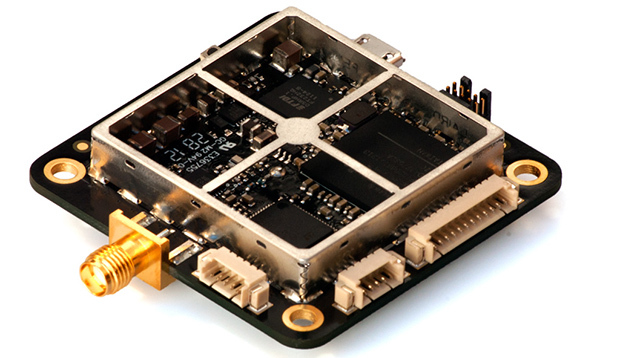
\includegraphics[width=6cm]{Figures/gps.jpg}
			\caption{GPS Piksi v2.3.1}
			\label{fig:GPS}
		\end{figure}
		
		O console foi instalado, o GPS foi conectado na USB do computador e a antena devidamente acoplada. Essa versão em específico precisa de quatro satélites para realizar os cálculos de coordenadas, e em ambientes fechados, a recepção de sinal é bastante degradada. Para contornar essa situação, o dispositivo foi iniciado em modo de simulação em seu console, mostrando assim, os dados de longitude e latitude.
		
		Posteriormente, a antena foi levada a um ambiente externo e verificou o funcionamento do GPS fora do modo de simulação.    
		
		\item IMU
		
		A IMU Mti-1, fabricado pela Xsens, possui um console que é disponibilizado no próprio pendrive de instalação que vem junto ao sensor.
		
		\begin{figure}[!ht]
			\centering
			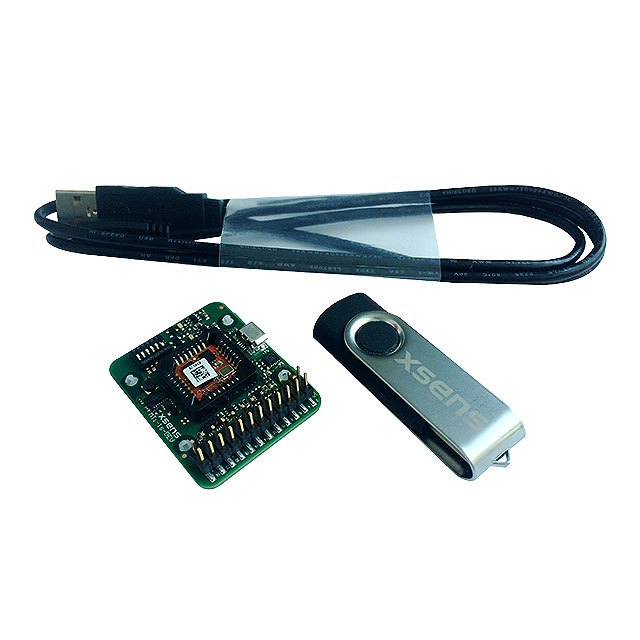
\includegraphics[width=8cm]{Figures/imu.jpg}
			\caption{IMU Xsens Mti-1}
			\label{fig:IMU}
		\end{figure}
		
		Com o console instalado, foi apenas necessário conectar a IMU a uma das portas USB do computador. Na própria interface gráfica já aparece as informações de orientação do dispositivo, informando a orientação nos três eixos de referência e velocidade angular.
	\end{itemize}
	
		%--------- NEW SECTION ----------------------
		\subsection{Integração dos sensores com ROS}
		\label{sec:rosinte}
		
		Após os testes unitários de cada sensor, deu-se inicio à integração dos sensores no ambiente ROS para construção do sistema de Percepção. A descrição da metodologia empregada para embarcar cada um dos sensores no framework de robótica está mostrada nos tópicos abaixo.
		
		\begin{itemize}

		\item Phidgets
		
		Após a fase de testes unitários, foi necessário desenvolver o \textit{package} de comunicação da phidgets no ROS. Esse \textit{package} é responsável pela aquisição dos dados de todos os sensores analógicos e digitais conectados a Phidgets.
		
		Os nós foram desenvolvidos utilizando como base o módulo \textit{python} da Phidgets. Ele consiste em uma classe e cada objeto desta, representa um componente conectado a placa de interface. Ao declarar o objeto, se faz necessário informar o canal, o nome do dispositivo, o tipo de porta (digital ou analógico) e o nome do tópico a ser disponibilizado os dados. 
		
		No construtor da classe os dados referentes aos dispositivos são coletados e um \textit{publisher} do ROS é inicializado. Este  \textit{publisher} faz com que periodicamente os dados de tensão(canais analógicos) ou status da porta(canais digitais) sejam coletados e disponibilizados no tópico escolhido pelo usuário. 
		
		No script original foram criados seis objetos da classe no \textit{main loop}, correspondentes aos cinco sensores de proximidade conectados a portas digitais e ao sonar conectado na porta analógica.
		
		\item Smart Charger
		
		O script utilizado no teste unitário para receber os dados provenientes do \textit{smart charger} no computador foi utilizado como base para a construção do nó no ambiente ROS.
		
		O nó funciona enviando um \textit{byte} pré-definido para dar início ao processo de transmissão de dados da bateria. A recepção do \textit{byte} pela Nucleo L432KC inicia a leitura dos dados da bateria, como mostrado no tópico anterior. Logo após isso, ocorre o envio das informações em sequência para o computador, como pode ser visto abaixo:
		
		\begin{figure}[!ht]
			\centering
			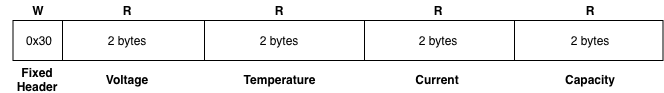
\includegraphics[width=16cm]{Figures/batt_protocol_2.png}
			\caption{Mensagem entre a Nucleo L432KC e o nó referente às baterias}
			\label{fig:battprotocol2}
		\end{figure}
		
		No nó do ROS essas informações são recebidas via serial e convertidas para sua devidas unidades segundo o \textit{datasheet} do fabricante. Esses dados são colocados em um formato de mensagem chamado de Battery e publicadas em um tópico do ROS. O nó criado para a \textit{smart charger} está mostrado no anexo XX.
		
		\item Câmera Térmica
		
		A integração da câmera no ROS foi feita em duas etapas, que na prática foram representadas como dois nós:
		
		\begin{itemize}
			\item O primeiro com objetivo da aquisição dos dados da câmera e sua disponibilização em um tópico.
			\item O segundo nó é responsável por todo o tratamento da imagem e detecção dos pontos quentes.
		\end{itemize}
		
		Para a aquisição dos dados, no primeiro nó, foi utilizado basicamente o mesmo algoritmo que no teste unitário, porém com a integração das bibliotecas do ROS para publicar os \textit{frames} em forma de \textit{Numpy arrays} em seus devido tópico.
		
		No segundo nó foi utilizado a biblioteca OpenCV para realizar o processamento da imagem. Primeiramente, o frame disponibilizado pelo nó de aquisição é adquirido subscrevendo do seu respectivo tópico. Para retirar o aspecto "pixelado" da imagem da câmera, devido a sua baixa resolução (80x60 pixeis), foi necessário realizar uma interpolação cúbica para redimensionar a imagem para uma resolução de (400x300 pixeis), obtendo assim uma imagem mais detalhada. 
		
		Com a imagem já redimensionada, é aplicado um filtro \textit{blur} para eliminar altas frequências que podem interferir na binarização (\textit{thresholding}) que será feita na imagem.
		
		Após o filtro, o frame é binarizado com o objetivo de facilitar a identificação dos pontos quentes através de um algoritmo de busca de contornos.
		
		O esquemático abaixo mostra simplificadamente o processo de tratamento da imagem.
		
		\begin{figure}[!ht]
			\centering
			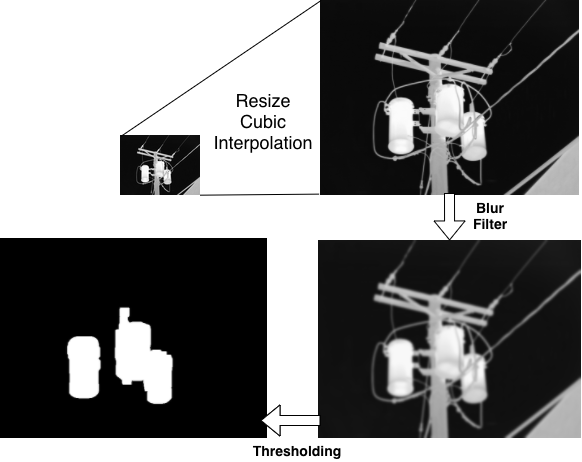
\includegraphics[width=14cm]{Figures/image_proc.png}
			\caption{Esquemático do processamento da imagem} \label{imgproc}
		\end{figure}
		
		\item GPS
		
		Para o GPS, foi utilizado um driver disponibilizado no GitHub por \citeonline{ethz} com licensa livre para embarcar o dispositivo no ROS.
		
		O \textit{package} possui nós que publicam em tópicos as informações de coordenadas obtidas do GPS.
		
		\item IMU
		
		Foi utilizado o driver da IMU disponibilizada pela própria fabricante Xsens para embarcar a IMU no ROS. O driver de licença livre é disponibilizado no GitHub da própria empresa.
		\end{itemize}
		
		%--------- NEW SECTION ----------------------
	
	\subsection{Interface do Usuário}
	\label{sec:ui}
	
	A interface do usuário é uma forma de expor graficamente as variáveis mais importantes do sistema robótico e quais atividades estão sendo executadas. Ela permite dar previsibilidade ao usuário do comportamento do sistema. 
	
	No ELIR a interface do usuário tem o papel de informar cinco características principais:
	
	\begin{itemize}
		\item \textit{System Integrity}
		\item \textit{Robot Status}
		\item \textit{Thermal view}
		\item \textit{Ocurrences}
		\item \textit{Actuators Information}
	\end{itemize}
	
	No campo de \textit{System Integrity} são exibidos em tempo real as variáveis de grande impacto na eficiência e integridade do sistema. Por isso são informados os dados de temperatura, percentual de carga da bateria, consumo, localização e orientação do robô.
	
	O \textit{Robot Status Display} exibe o posicionamento das garras do robô na linha de transmissão. A coloração vermelha indica as garras foras da linha enquanto que a coloração verde indica as garras apoiadas na linha. Essa informação proveniente dos sensores de proximidade é de extrema importância para integridade física do robô.
	
	O \textit{Thermal View} exibe em  tempo real os frames da câmera IR, permitindo o usuário acompanhar a detecção de pontos quentes e visualizar o perfil de temperatura da área exibida. 
	
	O campo de \textit{Ocurrences} mostra as principais ocorrências daquele momento, mostrando eventos de sobretemperatura, sobrecorrente, detecção de pontos quentes e detecção de objetos na área de servidão. Todos os eventos são mostra
	dos com data, horário e localização gps. 
	
	
	\section{Testes}
	Na fase de Testes as funcionalidades do sistema são colocadas a prova, para isso são efetuados testes de funcionamento com embasamento estatístico para comprovar que a funcionalidade está trabalhando da forma esperada. O resultado principal desta fase é um \textit{Logbook} contendo o resultado de cada teste efetuado. A descrição dos testes efetuados e os resultados obtidos estão mostrados em detalhes no capítulo 4.
	
	%importante: para palavras em outro idioma vc deve usar o itálico
	
	%--------- NEW SECTION ----------------------
	\section{Diagramas mecânicos}
	\label{sec:diagm}
	O sistema de Percepção em robôs muitas vezes é entendida como uma implementação em código das funcionalidades do sistema, desconsiderando o aporte mecânico envolvido. Contudo, o suporte mecânico para os sensores é um grande desafio a ser solucionado. 
	
	Neste projeto, houve a necessidade de suportes mecânicos por conta da limitação de espaço além de haver uma restrição imposta pelo cliente na modificação estrutural no protótipo. A descrição dos suportes mecânicos desenvolvidos para confrontar esse problema esta mostrada na próxima sessão.
	%
	%\subsection{Diagrama mecânico do ELIR}
	%shaushaus
	
	\section{Suporte dos sensores}
	
	Para  fixar  todos  os  sensores  e  componentes  eletrônicos  de  maneira  organizada foi desenhada uma estrutura em forma de prateleira  na qual é possível anexar a grande parte dos sensores do sistema de Percepção.
	
	A primeira prateleira comporta os sensores do sistema de georreferenciamento que são o GPS e a IMU. A prateleira central foi projetada para a placa de interface Nucleo F401RE que recebe os dados da câmera IR. Por último, na terceira prateleira fica a placa de interface Phidgets para reunir os dados dos diferentes componentes e enviar para a NUC que é a  unidade de processamento central do robô.
	
	As peças foram fabricadas utilizando impressão 3D e o seu desenho pode ser visto nas Figura \ref{Prateleira} e \ref{Prateleiracsensor} .
	
	\begin{figure}[h]
		\centering
		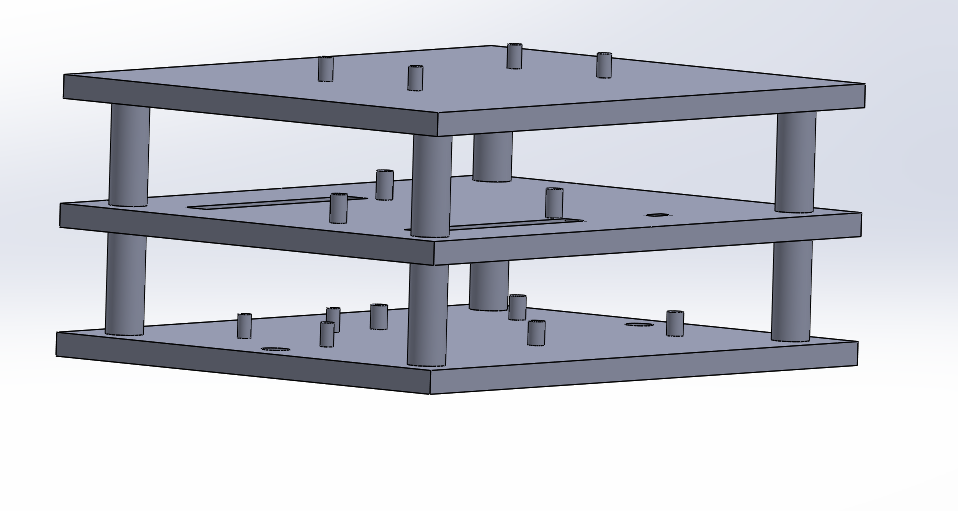
\includegraphics[width=14cm]{Figures/prateleira.png}
		\caption{Prateleira para suporte dos componentes eletrônicos} \label{Prateleira}
	\end{figure}
	
	%\begin{figure}[h]
	%	\centering
	%	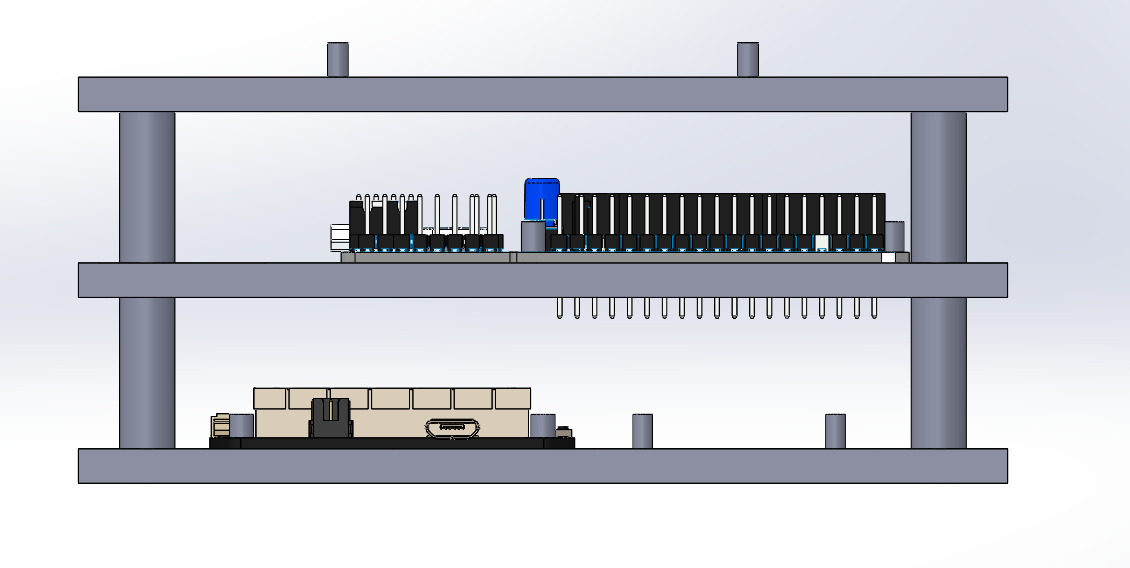
\includegraphics[width=16cm]{Figures/prateleiracsensores.png}
	%	\caption{Prateleira para suporte com sensores} \label{Prateleiracsensor}
	%\end{figure}
	
	
	A parte de gerenciamento enérgico do robô foi alocada em uma estrutura na parte inferior do mesmo. Esta estrutura foi projetada para comportar as baterias, a \textit{Smart Charger}, a \textit{Power Management} e a placa de interface Nucleo L432. O desenho dessa estrutura está mostrado na figura \ref{pecaaliment}.
	
	\begin{figure}[h]
		\centering
		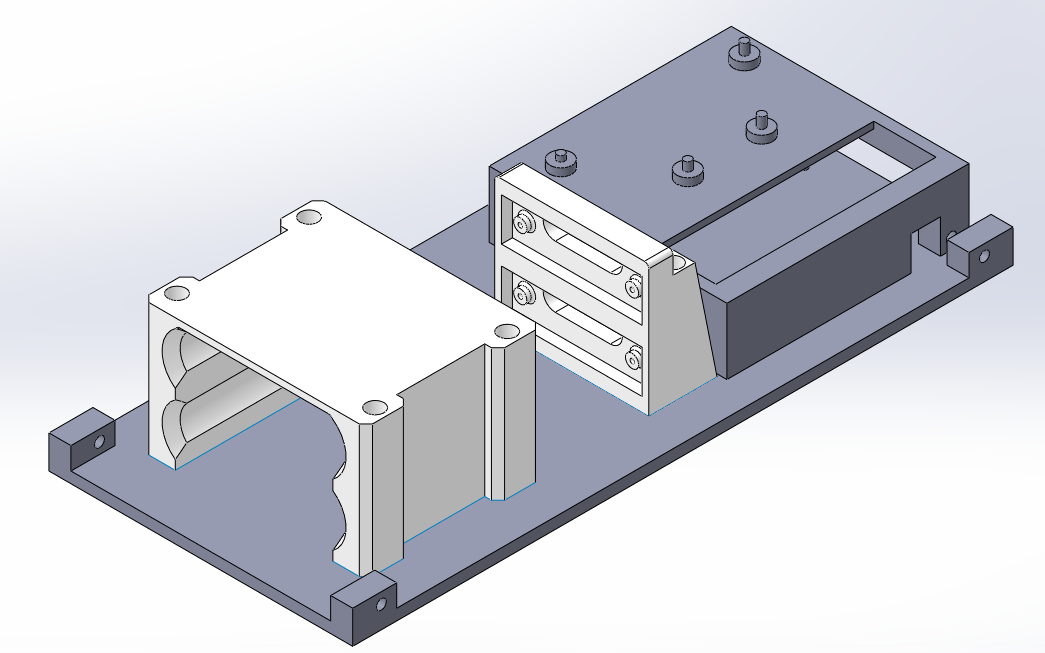
\includegraphics[width=14cm]{Figures/pecadebaixo.png}
		\caption{Prateleira para suporte dos componentes de alimentação} \label{pecaaliment}
	\end{figure}
	
	%--------- NEW SECTION ----------------------
	\section{Modelo esquemático de alimentação e comunicação}
	\label{sec:modesq}
	A alimentação do sistema é proveniente de duas baterias LiPo que fornecem tensão de alimentação em 14V. Todo o gerenciamento de energia do sistema é feita pela \textit{Power Management Board}, esta placa é responsável por distribuir a alimentação de entrada para os demais subsistemas da Percepção. 
	
	A placa de interface Phidgets além de funcionar como \textit{hub} para uma grande parte dos sensores também é responsável por compatibilizar o nível de tensão para os componentes eletrônicos, fornecendo 5V para as placas microprocessadas, sensores e a alimentação de todas as portas USBs. 
	
	A comunicação entre os sistemas da Percepção ocorrem na maior parte  através da Phidgets, já que esta placa de interface concentra as informações oriundas de suas portas USB, entrada digitais e entradas analógicas em uma única porta USB para a unidade central de processamento.
	
	A câmera térmica e a os dynamixels possuem portas exclusivas de comunicação com a unidade central devido seu grau de criticidade.
	
	\section{Diagramas elétricos e eletrônicos}
	\label{sec:diage}
	O diagrama elétrico do sistema está disponível no apêndice \ref{Append:diagele}. Neste diagrama encontram-se todas as conexões elétricas e de comunicação bem como as especificações de conectores e cabos utilizados no projeto.
	
	O esquemático eletrônico realizado pela equipe foi uma placa hub de 5V para alimentação dos sensores de proximidade, visto que a Phidgets possui apenas umas saída de tensão em 5V disponibilizada.
	
	Nesta placa foram colocados os \textit{pin headers} para cada sensor de proximidade, fornecendo alimentação e disponibilizando os pinos digitais dos sensores em um conector Molex.
	
	O esquemático eletrônico e \textit{board} estão mostrados no anexo \ref{Append:diagele}.

